% ===========================================================================
%  TikuOS — TikuKits ML: Linear Regression for Embedded Systems
%  Beamer Presentation
% ===========================================================================
\documentclass[aspectratio=169, 10pt]{beamer}

% ---- Theme ----------------------------------------------------------------
\usetheme{Madrid}
\usecolortheme{whale}
\setbeamertemplate{navigation symbols}{}
\setbeamertemplate{footline}{%
  \leavevmode\hbox{%
    \begin{beamercolorbox}[wd=.33\paperwidth,ht=2.5ex,dp=1ex,center]{author in head/foot}%
      \usebeamerfont{author in head/foot}\insertshortauthor
    \end{beamercolorbox}%
    \begin{beamercolorbox}[wd=.34\paperwidth,ht=2.5ex,dp=1ex,center]{title in head/foot}%
      \usebeamerfont{title in head/foot}\insertshorttitle
    \end{beamercolorbox}%
    \begin{beamercolorbox}[wd=.33\paperwidth,ht=2.5ex,dp=1ex,right]{date in head/foot}%
      \usebeamerfont{date in head/foot}\insertshortdate{}\hspace*{2em}%
      \insertframenumber{}/\inserttotalframenumber\hspace*{2ex}
    \end{beamercolorbox}}%
  \vskip0pt%
}

% ---- Packages -------------------------------------------------------------
\usepackage{listings}
\usepackage{graphicx}
\usepackage{hyperref}
\usepackage{booktabs}
\usepackage{multirow}
\usepackage{tikz}
\usetikzlibrary{arrows.meta, positioning, shapes.geometric, calc,
                decorations.pathreplacing, fit}
\usepackage{amsmath}

% ---- Code listing style ---------------------------------------------------
\lstset{
  basicstyle=\ttfamily\scriptsize,
  keywordstyle=\color{blue}\bfseries,
  commentstyle=\color{gray},
  stringstyle=\color{red!70!black},
  showstringspaces=false,
  breaklines=true,
  frame=single,
  rulecolor=\color{black!30},
  backgroundcolor=\color{blue!3},
  tabsize=4,
}
\lstdefinestyle{cstyle}{
  language=C,
  morekeywords={uint8_t,uint16_t,uint32_t,int32_t,int64_t,
                tiku_kits_ml_elem_t,
                TIKU_KITS_ML_OK,TIKU_KITS_ML_ERR_NULL,
                TIKU_KITS_ML_ERR_SIZE,TIKU_KITS_ML_ERR_PARAM,
                TIKU_KITS_ML_ERR_SINGULAR,TIKU_KITS_ML_ERR_OVERFLOW,
                TIKU_KITS_ML_ELEM_TYPE,TIKU_KITS_ML_LINREG_SHIFT,
                NULL},
}

% ---- Metadata -------------------------------------------------------------
\title[TikuKits ML]{TikuKits ML: Linear Regression for Embedded Systems}
\subtitle{Simple. Ubiquitous. Intelligence, Everywhere.}
\author[Ambuj Varshney]{Ambuj Varshney \\ \texttt{ambuj@tiku-os.org}}
\date{\today}

% ===========================================================================
\begin{document}

% ---------------------------------------------------------------------------
\begin{frame}
\titlepage
\end{frame}

% ---------------------------------------------------------------------------
\begin{frame}{Outline}
\tableofcontents
\end{frame}

% ===========================================================================
\section{Motivation}
% ===========================================================================

\begin{frame}{Why ML on Ultra-Low-Power MCUs?}
\begin{columns}[T]
\begin{column}{0.48\textwidth}
\begin{block}{Embedded Use Cases}
\begin{itemize}
  \item \textbf{Sensor calibration} --- map raw ADC to physical units
  \item \textbf{Trend detection} --- detect drift in readings over time
  \item \textbf{Prediction} --- estimate battery charge from voltage
  \item \textbf{Anomaly flagging} --- R$^2$ drop signals sensor failure
\end{itemize}
\end{block}

\begin{block}{Constraints}
\begin{itemize}
  \item No FPU (16-bit MSP430)
  \item No heap allocation
  \item Limited RAM (2--8\,KB)
  \item Every $\mu$J counts
\end{itemize}
\end{block}
\end{column}

\begin{column}{0.48\textwidth}
\begin{center}
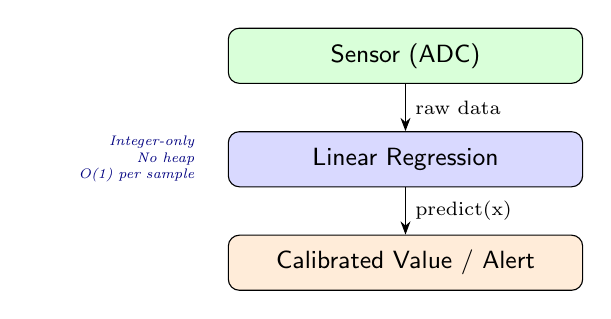
\begin{tikzpicture}[
    >=Stealth, node distance=0.5cm
  ]
  \node[draw, rounded corners, minimum height=0.7cm,
        text centered, font=\small\sffamily, fill=green!15,
        minimum width=4.5cm] (sensor) {Sensor (ADC)};
  \node[draw, rounded corners, minimum height=0.7cm,
        text centered, font=\small\sffamily, fill=blue!15,
        minimum width=4.5cm, below=0.6cm of sensor] (linreg)
    {Linear Regression};
  \node[draw, rounded corners, minimum height=0.7cm,
        text centered, font=\small\sffamily, fill=orange!15,
        minimum width=4.5cm, below=0.6cm of linreg] (output)
    {Calibrated Value / Alert};
  \draw[->] (sensor) -- node[right, font=\scriptsize] {raw data} (linreg);
  \draw[->] (linreg) -- node[right, font=\scriptsize] {predict(x)} (output);

  \node[left=0.3cm of linreg, font=\tiny\itshape, text=blue!50!black,
        text width=2cm, align=right] {Integer-only\\No heap\\O(1) per sample};
\end{tikzpicture}
\end{center}

\vspace{0.5em}
\begin{alertblock}{Design Goal}
Bring linear regression to devices with \textbf{no floating point},
using only static memory and integer arithmetic.
\end{alertblock}
\end{column}
\end{columns}
\end{frame}

% ===========================================================================
\section{Architecture}
% ===========================================================================

\begin{frame}{ML Kit in the TikuKits Ecosystem}
\begin{center}
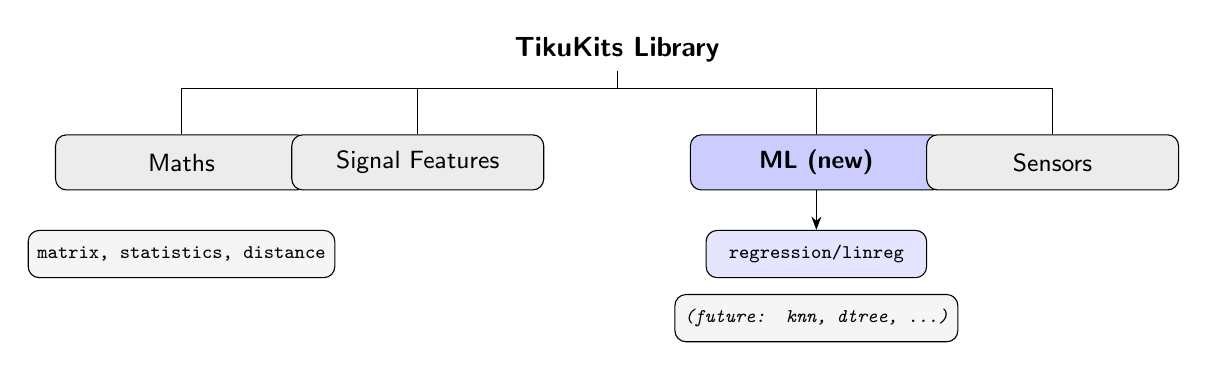
\begin{tikzpicture}[
    >=Stealth, node distance=0.4cm
  ]

  % TikuKits parent
  \node[font=\normalsize\sffamily\bfseries] (title) {TikuKits Library};

  % Existing kits
  \node[draw, rounded corners, minimum height=0.7cm,
        text centered, font=\small\sffamily, fill=gray!15,
        minimum width=3.2cm, below left=0.8cm and 2.5cm of title] (maths)
    {Maths};
  \node[draw, rounded corners, minimum height=0.7cm,
        text centered, font=\small\sffamily, fill=gray!15,
        minimum width=3.2cm, below left=0.8cm and -0.5cm of title] (sig)
    {Signal Features};
  \node[draw, rounded corners, minimum height=0.7cm,
        text centered, font=\small\sffamily, fill=blue!20,
        minimum width=3.2cm, below right=0.8cm and -0.5cm of title] (ml)
    {\textbf{ML (new)}};
  \node[draw, rounded corners, minimum height=0.7cm,
        text centered, font=\small\sffamily, fill=gray!15,
        minimum width=3.2cm, below right=0.8cm and 2.5cm of title] (sensor)
    {Sensors};

  % ML sub-modules
  \node[draw, rounded corners, minimum height=0.6cm,
        text centered, font=\scriptsize\ttfamily, fill=blue!10,
        minimum width=2.8cm, below=0.5cm of ml] (linreg)
    {regression/linreg};
  \node[draw, rounded corners, minimum height=0.6cm,
        text centered, font=\scriptsize\ttfamily\itshape, fill=gray!8,
        minimum width=2.8cm, below=0.2cm of linreg]
    (future1) {(future: knn, dtree, ...)};

  % Maths sub-modules
  \node[draw, rounded corners, minimum height=0.6cm,
        text centered, font=\scriptsize\ttfamily, fill=gray!8,
        minimum width=2.8cm, below=0.5cm of maths]
    {matrix, statistics, distance};

  \draw[-] (title) -- ++(0,-0.5) -| (maths);
  \draw[-] (title) -- ++(0,-0.5) -| (sig);
  \draw[-] (title) -- ++(0,-0.5) -| (ml);
  \draw[-] (title) -- ++(0,-0.5) -| (sensor);
  \draw[->] (ml) -- (linreg);
\end{tikzpicture}
\end{center}

\vspace{0.3em}
\begin{table}
\centering
\small
\begin{tabular}{@{}llp{6cm}@{}}
\toprule
\textbf{File} & \textbf{Role} \\
\midrule
\texttt{ml/tiku\_kits\_ml.h} & Common return codes for all ML sub-modules \\
\texttt{ml/regression/tiku\_kits\_ml\_linreg.h} & Linear regression API \\
\texttt{ml/regression/tiku\_kits\_ml\_linreg.c} & Implementation \\
\bottomrule
\end{tabular}
\end{table}
\end{frame}

% ===========================================================================
\section{Linear Regression Theory}
% ===========================================================================

\begin{frame}{Ordinary Least Squares (OLS)}
\begin{columns}[T]
\begin{column}{0.48\textwidth}
\textbf{Model:} \quad $y = \beta_1 x + \beta_0$

\vspace{0.5em}
\textbf{Given} $n$ data points $(x_i, y_i)$, the OLS solution
minimises $\sum (y_i - \hat{y}_i)^2$:

\vspace{0.3em}
\[
  \beta_1 = \frac{n \sum x_i y_i - \sum x_i \sum y_i}
                 {n \sum x_i^2 - \left(\sum x_i\right)^2}
\]

\[
  \beta_0 = \frac{\sum y_i - \beta_1 \sum x_i}{n}
\]

\vspace{0.3em}
\textbf{Prediction:}
\[
  \hat{y} = \beta_1 x + \beta_0
\]

\textbf{Goodness of fit:}
\[
  R^2 = \frac{\left(n S_{xy} - S_x S_y\right)^2}
             {\left(n S_{xx} - S_x^2\right)\left(n S_{yy} - S_y^2\right)}
\]
\end{column}

\begin{column}{0.48\textwidth}
\begin{center}
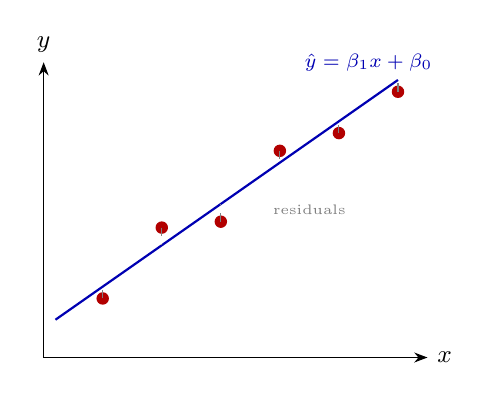
\begin{tikzpicture}[>=Stealth, scale=0.75]
  % Axes
  \draw[->] (0,0) -- (6.5,0) node[right] {\small $x$};
  \draw[->] (0,0) -- (0,5) node[above] {\small $y$};

  % Best-fit line: y = 0.7x + 0.5
  \draw[thick, blue!70!black] (0.2, 0.64) -- (6, 4.7);

  % Data points
  \fill[red!70!black] (1, 1.0) circle (3pt);
  \fill[red!70!black] (2, 2.2) circle (3pt);
  \fill[red!70!black] (3, 2.3) circle (3pt);
  \fill[red!70!black] (4, 3.5) circle (3pt);
  \fill[red!70!black] (5, 3.8) circle (3pt);
  \fill[red!70!black] (6, 4.5) circle (3pt);

  % Residuals
  \draw[dashed, gray] (1, 1.0) -- (1, 1.2);
  \draw[dashed, gray] (2, 2.2) -- (2, 1.9);
  \draw[dashed, gray] (3, 2.3) -- (3, 2.6);
  \draw[dashed, gray] (4, 3.5) -- (4, 3.3);
  \draw[dashed, gray] (5, 3.8) -- (5, 4.0);
  \draw[dashed, gray] (6, 4.5) -- (6, 4.7);

  % Labels
  \node[font=\scriptsize, blue!70!black] at (5.5, 5) {$\hat{y} = \beta_1 x + \beta_0$};
  \node[font=\tiny, gray] at (4.5, 2.5) {residuals};
\end{tikzpicture}
\end{center}

\vspace{0.5em}
\begin{block}{Key Insight}
OLS only needs \textbf{five running sums}:\\
$S_x$, $S_y$, $S_{xx}$, $S_{xy}$, $S_{yy}$.\\
No sample buffer required --- O(1) memory.
\end{block}
\end{column}
\end{columns}
\end{frame}

% ---------------------------------------------------------------------------
\begin{frame}{Integer-Only Implementation Strategy}
\begin{columns}[T]
\begin{column}{0.48\textwidth}
\begin{block}{Problem}
Slope and intercept are typically \textbf{fractional}.\\
MSP430 has no FPU --- division truncates to zero.\\
$\beta_1 = 1.5 \rightarrow$ \texttt{int} gives 1 (33\% error).
\end{block}

\vspace{0.3em}
\begin{block}{Solution: Fixed-Point Q-Format}
Scale by $2^{\text{shift}}$ before dividing:
\[
  \text{slope\_q} = \frac{\text{num} \ll \text{shift}}{\text{den}}
\]
With \texttt{shift=8}, resolution $= \frac{1}{256} \approx 0.004$.\\[0.3em]
To recover real value: $\text{slope} = \frac{\text{slope\_q}}{256}$.
\end{block}
\end{column}

\begin{column}{0.48\textwidth}
\begin{block}{Overflow Prevention}
\begin{itemize}
  \item All accumulators use \texttt{int64\_t}
  \item Products $x \cdot y$ computed as\\
        \texttt{(int64\_t)x * (int64\_t)y}
  \item Safe for \texttt{int32\_t} inputs:\\
        $2^{31} \times 2^{31} = 2^{62} < 2^{63}$
\end{itemize}
\end{block}

\vspace{0.3em}
\begin{block}{Prediction Without Scaling}
\texttt{predict()} returns values in the \textbf{original integer
domain} --- no Q-format decoding needed:
\[
  \hat{y} = \frac{\text{num} \cdot (n \cdot x - S_x) + S_y \cdot \text{den}}{n \cdot \text{den}}
\]
\end{block}
\end{column}
\end{columns}
\end{frame}

% ===========================================================================
\section{Data Structure}
% ===========================================================================

\begin{frame}[fragile]{The \texttt{tiku\_kits\_ml\_linreg} Structure}
\begin{columns}[T]
\begin{column}{0.48\textwidth}
\begin{lstlisting}[style=cstyle,
  title={ml/regression/tiku\_kits\_ml\_linreg.h}]
struct tiku_kits_ml_linreg {
    int64_t sum_x;   /* Sum of x       */
    int64_t sum_y;   /* Sum of y       */
    int64_t sum_xx;  /* Sum of x*x     */
    int64_t sum_xy;  /* Sum of x*y     */
    int64_t sum_yy;  /* Sum of y*y     */
    uint16_t n;      /* Data points    */
    uint8_t shift;   /* Q-format bits  */
};
\end{lstlisting}

\vspace{0.3em}
\textbf{Memory footprint:}\\
$5 \times 8 + 2 + 1 = 43$ bytes per model.\\
All statically allocated --- no heap.
\end{column}

\begin{column}{0.48\textwidth}
\textbf{Streaming accumulator pattern:}
\begin{center}
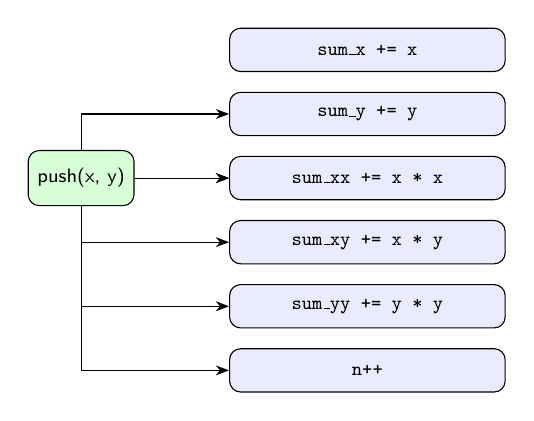
\begin{tikzpicture}[
    >=Stealth, node distance=0.25cm
  ]
  \node[draw, rounded corners, minimum height=0.55cm,
        text centered, font=\scriptsize\ttfamily, fill=blue!8,
        minimum width=3.5cm] (sx) {sum\_x += x};
  \node[draw, rounded corners, minimum height=0.55cm,
        text centered, font=\scriptsize\ttfamily, fill=blue!8,
        minimum width=3.5cm, below=of sx] (sy) {sum\_y += y};
  \node[draw, rounded corners, minimum height=0.55cm,
        text centered, font=\scriptsize\ttfamily, fill=blue!8,
        minimum width=3.5cm, below=of sy] (sxx) {sum\_xx += x * x};
  \node[draw, rounded corners, minimum height=0.55cm,
        text centered, font=\scriptsize\ttfamily, fill=blue!8,
        minimum width=3.5cm, below=of sxx] (sxy) {sum\_xy += x * y};
  \node[draw, rounded corners, minimum height=0.55cm,
        text centered, font=\scriptsize\ttfamily, fill=blue!8,
        minimum width=3.5cm, below=of sxy] (syy) {sum\_yy += y * y};
  \node[draw, rounded corners, minimum height=0.55cm,
        text centered, font=\scriptsize\ttfamily, fill=blue!8,
        minimum width=3.5cm, below=of syy] (nn) {n++};

  \node[draw, rounded corners, fill=green!15,
        font=\scriptsize\sffamily, left=1.2cm of sxx,
        minimum height=0.7cm] (push) {push(x, y)};

  \draw[->] (push) -- (sx.west |- push);
  \draw[->] (push) |- (sy);
  \draw[->] (push) -- (sxx);
  \draw[->] (push) |- (sxy);
  \draw[->] (push) |- (syy);
  \draw[->] (push) |- (nn);
\end{tikzpicture}
\end{center}
Each \texttt{push()} is \textbf{O(1)} --- five multiply-add operations.
\end{column}
\end{columns}
\end{frame}

% ===========================================================================
\section{Return Codes}
% ===========================================================================

\begin{frame}[fragile]{ML Kit Return Codes}
\begin{columns}[T]
\begin{column}{0.48\textwidth}
\begin{lstlisting}[style=cstyle, title={ml/tiku\_kits\_ml.h}]
#define TIKU_KITS_ML_OK            0
#define TIKU_KITS_ML_ERR_NULL    (-1)
#define TIKU_KITS_ML_ERR_SIZE    (-2)
#define TIKU_KITS_ML_ERR_PARAM   (-3)
#define TIKU_KITS_ML_ERR_SINGULAR (-4)
#define TIKU_KITS_ML_ERR_OVERFLOW (-5)
\end{lstlisting}

\vspace{0.3em}
Defined in the \textbf{kit-level common header} ---
shared by all ML sub-modules (linear regression, and
future modules like kNN, decision tree, etc.).
\end{column}

\begin{column}{0.48\textwidth}
\begin{table}
\centering
\small
\begin{tabular}{@{}lp{4.5cm}@{}}
\toprule
\textbf{Code} & \textbf{Meaning} \\
\midrule
\texttt{OK}       & Operation succeeded \\
\texttt{ERR\_NULL} & NULL pointer passed \\
\texttt{ERR\_SIZE} & Fewer than 2 data points \\
\texttt{ERR\_PARAM} & Invalid parameter (e.g. shift > 30) \\
\texttt{ERR\_SINGULAR} & All x values identical (zero variance) \\
\texttt{ERR\_OVERFLOW} & Arithmetic overflow \\
\bottomrule
\end{tabular}
\end{table}
\end{column}
\end{columns}
\end{frame}

% ===========================================================================
\section{API Reference}
% ===========================================================================

\begin{frame}[fragile]{Complete API}
\begin{table}
\centering
\small
\begin{tabular}{@{}lp{8.5cm}@{}}
\toprule
\textbf{Function} & \textbf{Description} \\
\midrule
\texttt{tiku\_kits\_ml\_linreg\_init(lr, shift)}
  & Initialize model with Q-format precision (shift = 0..30) \\
\texttt{tiku\_kits\_ml\_linreg\_reset(lr)}
  & Clear all data points, preserve shift \\
\texttt{tiku\_kits\_ml\_linreg\_push(lr, x, y)}
  & Stream a data point --- O(1), 5 multiply-adds \\
\midrule
\texttt{tiku\_kits\_ml\_linreg\_slope(lr, \&result)}
  & Fitted slope $\times 2^{\text{shift}}$ (Q-format) \\
\texttt{tiku\_kits\_ml\_linreg\_intercept(lr, \&result)}
  & Fitted intercept $\times 2^{\text{shift}}$ (Q-format) \\
\texttt{tiku\_kits\_ml\_linreg\_predict(lr, x, \&result)}
  & Predicted $\hat{y}$ in original integer scale \\
\texttt{tiku\_kits\_ml\_linreg\_r2(lr, \&result)}
  & $R^2 \times 2^{\text{shift}}$; range $[0, 2^{\text{shift}}]$ \\
\midrule
\texttt{tiku\_kits\_ml\_linreg\_count(lr)}
  & Number of data points pushed \\
\bottomrule
\end{tabular}
\end{table}

\vspace{0.3em}
\begin{alertblock}{Minimum Data Requirement}
\texttt{slope()}, \texttt{intercept()}, \texttt{predict()}, and \texttt{r2()}
require $\geq 2$ data points with distinct $x$ values.
Returns \texttt{ERR\_SIZE} or \texttt{ERR\_SINGULAR} otherwise.
\end{alertblock}
\end{frame}

% ===========================================================================
\section{Configuration}
% ===========================================================================

\begin{frame}[fragile]{Compile-Time Configuration}
\begin{columns}[T]
\begin{column}{0.48\textwidth}
\begin{lstlisting}[style=cstyle,
  title={Configurable element type}]
/* Default: int32_t (no FPU needed) */
#ifndef TIKU_KITS_ML_ELEM_TYPE
#define TIKU_KITS_ML_ELEM_TYPE int32_t
#endif

typedef TIKU_KITS_ML_ELEM_TYPE
    tiku_kits_ml_elem_t;

/* Override for tight memory: */
#define TIKU_KITS_ML_ELEM_TYPE int16_t
#include "tiku_kits_ml_linreg.h"
\end{lstlisting}
\end{column}

\begin{column}{0.48\textwidth}
\begin{lstlisting}[style=cstyle,
  title={Configurable Q-format precision}]
/* Default: 8 fractional bits */
#ifndef TIKU_KITS_ML_LINREG_SHIFT
#define TIKU_KITS_ML_LINREG_SHIFT 8
#endif

/* Or set at runtime: */
tiku_kits_ml_linreg_init(&lr, 12);
/* 12-bit: resolution ~0.00024 */
\end{lstlisting}

\vspace{0.3em}
\begin{table}
\centering
\scriptsize
\begin{tabular}{@{}rrr@{}}
\toprule
\textbf{Shift} & \textbf{Scale} & \textbf{Resolution} \\
\midrule
4  & 16     & 0.0625 \\
8  & 256    & 0.0039 \\
12 & 4096   & 0.00024 \\
16 & 65536  & 0.000015 \\
\bottomrule
\end{tabular}
\end{table}
\end{column}
\end{columns}
\end{frame}

% ===========================================================================
\section{Implementation Details}
% ===========================================================================

\begin{frame}[fragile]{Core: Push \& Slope}
\begin{columns}[T]
\begin{column}{0.48\textwidth}
\begin{lstlisting}[style=cstyle,
  title={tiku\_kits\_ml\_linreg.c --- push}]
int tiku_kits_ml_linreg_push(
    struct tiku_kits_ml_linreg *lr,
    tiku_kits_ml_elem_t x,
    tiku_kits_ml_elem_t y)
{
    if (lr == NULL)
        return TIKU_KITS_ML_ERR_NULL;

    lr->sum_x  += (int64_t)x;
    lr->sum_y  += (int64_t)y;
    lr->sum_xx += (int64_t)x * (int64_t)x;
    lr->sum_xy += (int64_t)x * (int64_t)y;
    lr->sum_yy += (int64_t)y * (int64_t)y;
    lr->n++;

    return TIKU_KITS_ML_OK;
}
\end{lstlisting}
\end{column}

\begin{column}{0.48\textwidth}
\begin{lstlisting}[style=cstyle,
  title={tiku\_kits\_ml\_linreg.c --- slope}]
int tiku_kits_ml_linreg_slope(
    const struct tiku_kits_ml_linreg *lr,
    int32_t *result)
{
    int64_t num, den;
    int rc;

    if (lr == NULL || result == NULL)
        return TIKU_KITS_ML_ERR_NULL;

    rc = slope_parts(lr, &num, &den);
    if (rc != TIKU_KITS_ML_OK)
        return rc;

    /* Fixed-point scaling */
    *result = (int32_t)(
        (num << lr->shift) / den);
    return TIKU_KITS_ML_OK;
}
\end{lstlisting}
\end{column}
\end{columns}
\end{frame}

% ---------------------------------------------------------------------------
\begin{frame}[fragile]{Core: Predict \& R-Squared}
\begin{columns}[T]
\begin{column}{0.48\textwidth}
\begin{lstlisting}[style=cstyle,
  title={predict --- returns original scale}]
int tiku_kits_ml_linreg_predict(
    const struct tiku_kits_ml_linreg *lr,
    tiku_kits_ml_elem_t x,
    tiku_kits_ml_elem_t *result)
{
    int64_t num, den, y_num;
    /* ... NULL/size checks ... */

    /*
     * y = (num*(n*x - Sx) + Sy*den)
     *     / (n * den)
     *
     * No fixed-point decoding needed.
     */
    y_num = num * ((int64_t)lr->n
                * (int64_t)x - lr->sum_x)
            + lr->sum_y * den;

    *result = (tiku_kits_ml_elem_t)(
        y_num / ((int64_t)lr->n * den));
    return TIKU_KITS_ML_OK;
}
\end{lstlisting}
\end{column}

\begin{column}{0.48\textwidth}
\begin{lstlisting}[style=cstyle,
  title={R-squared --- goodness of fit}]
int tiku_kits_ml_linreg_r2(
    const struct tiku_kits_ml_linreg *lr,
    int32_t *result)
{
    int64_t num, den, ss_yy;
    /* ... NULL/size checks ... */

    /* SS_yy = n*Syy - Sy^2 */
    ss_yy = (int64_t)lr->n * lr->sum_yy
            - lr->sum_y * lr->sum_y;

    if (ss_yy == 0)
        return TIKU_KITS_ML_ERR_SINGULAR;

    /* R^2 = num^2 / (den * ss_yy)
     * scaled by (1 << shift)       */
    *result = (int32_t)(
        ((num / den) * num << lr->shift)
        / ss_yy);

    /* Clamp to [0, 1<<shift] */
    if (*result > (int32_t)(1<<lr->shift))
        *result = (int32_t)(1<<lr->shift);
    if (*result < 0) *result = 0;

    return TIKU_KITS_ML_OK;
}
\end{lstlisting}
\end{column}
\end{columns}
\end{frame}

% ---------------------------------------------------------------------------
\begin{frame}[fragile]{Internal Helper: Slope Decomposition}
\begin{lstlisting}[style=cstyle,
  title={slope\_parts --- shared by slope, intercept, predict, r2}]
static int slope_parts(const struct tiku_kits_ml_linreg *lr,
                       int64_t *num, int64_t *den)
{
    int64_t d;

    if (lr->n < 2)
        return TIKU_KITS_ML_ERR_SIZE;

    *num = (int64_t)lr->n * lr->sum_xy - lr->sum_x * lr->sum_y;

    d = (int64_t)lr->n * lr->sum_xx - lr->sum_x * lr->sum_x;
    if (d == 0)
        return TIKU_KITS_ML_ERR_SINGULAR;    /* all x values identical */

    *den = d;
    return TIKU_KITS_ML_OK;
}
\end{lstlisting}

\vspace{0.3em}
\begin{block}{Why a Helper?}
All four query functions (\texttt{slope}, \texttt{intercept}, \texttt{predict},
\texttt{r2}) need the same numerator and denominator decomposition.
Factoring it out avoids code duplication and ensures consistent error handling.
\end{block}
\end{frame}

% ===========================================================================
\section{Examples}
% ===========================================================================

\begin{frame}[fragile]{Example 1: Sensor Calibration}
\begin{lstlisting}[style=cstyle,
  title={examples/example\_ml\_linreg.c --- ADC to temperature}]
struct tiku_kits_ml_linreg lr;
int32_t slope_q, intercept_q, r2_q;
tiku_kits_ml_elem_t y_pred;

tiku_kits_ml_linreg_init(&lr, 8);

/* Calibration data: (raw_adc, temperature_deci_C) */
tiku_kits_ml_linreg_push(&lr, 100, 0);     /* 0.0 C */
tiku_kits_ml_linreg_push(&lr, 200, 100);   /* 10.0 C */
tiku_kits_ml_linreg_push(&lr, 300, 200);   /* 20.0 C */
tiku_kits_ml_linreg_push(&lr, 400, 300);   /* 30.0 C */
tiku_kits_ml_linreg_push(&lr, 500, 400);   /* 40.0 C */

tiku_kits_ml_linreg_slope(&lr, &slope_q);       /* 256 (1.0 Q8) */
tiku_kits_ml_linreg_intercept(&lr, &intercept_q); /* -25600 (-100.0 Q8) */
tiku_kits_ml_linreg_r2(&lr, &r2_q);             /* 256 (1.0 Q8, perfect) */

/* Convert a new ADC reading to temperature */
tiku_kits_ml_linreg_predict(&lr, 350, &y_pred);  /* y_pred = 250 (25.0 C) */
\end{lstlisting}
\end{frame}

% ---------------------------------------------------------------------------
\begin{frame}[fragile]{Example 2: Trend Detection}
\begin{columns}[T]
\begin{column}{0.52\textwidth}
\begin{lstlisting}[style=cstyle,
  title={Detect drift in sensor readings}]
struct tiku_kits_ml_linreg lr;
int32_t slope_q;

static const tiku_kits_ml_elem_t
    readings[] = {
    500, 502, 498, 505, 501, 507,
    503, 510, 506, 512, 508, 515,
    511, 518, 514, 521
};

tiku_kits_ml_linreg_init(&lr, 8);
for (i = 0; i < 16; i++)
    tiku_kits_ml_linreg_push(&lr,
        (tiku_kits_ml_elem_t)i,
        readings[i]);

tiku_kits_ml_linreg_slope(&lr, &slope_q);

if (slope_q > 25)       /* > ~0.1/sample */
    alert_upward_drift();
else if (slope_q < -25)
    alert_downward_drift();
\end{lstlisting}
\end{column}

\begin{column}{0.44\textwidth}
\begin{center}
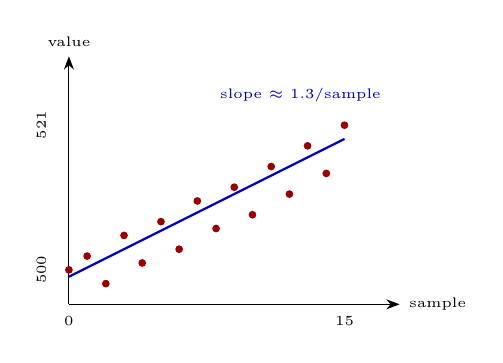
\begin{tikzpicture}[>=Stealth, scale=0.7]
  % Axes
  \draw[->] (0,0) -- (6,0) node[right] {\tiny sample};
  \draw[->] (0,0) -- (0,4.5) node[above] {\tiny value};

  % Data points (scaled: x/3, (y-495)/8)
  \fill[red!60!black] (0.0, 0.625) circle (2pt);
  \fill[red!60!black] (0.33, 0.875) circle (2pt);
  \fill[red!60!black] (0.67, 0.375) circle (2pt);
  \fill[red!60!black] (1.0, 1.25) circle (2pt);
  \fill[red!60!black] (1.33, 0.75) circle (2pt);
  \fill[red!60!black] (1.67, 1.5) circle (2pt);
  \fill[red!60!black] (2.0, 1.0) circle (2pt);
  \fill[red!60!black] (2.33, 1.875) circle (2pt);
  \fill[red!60!black] (2.67, 1.375) circle (2pt);
  \fill[red!60!black] (3.0, 2.125) circle (2pt);
  \fill[red!60!black] (3.33, 1.625) circle (2pt);
  \fill[red!60!black] (3.67, 2.5) circle (2pt);
  \fill[red!60!black] (4.0, 2.0) circle (2pt);
  \fill[red!60!black] (4.33, 2.875) circle (2pt);
  \fill[red!60!black] (4.67, 2.375) circle (2pt);
  \fill[red!60!black] (5.0, 3.25) circle (2pt);

  % Trend line
  \draw[thick, blue!70!black] (0, 0.5) -- (5.0, 3.0);
  \node[font=\tiny, blue!70!black] at (4.2, 3.8)
    {slope $\approx$ 1.3/sample};

  % Labels
  \node[font=\tiny] at (0, -0.3) {0};
  \node[font=\tiny] at (5.0, -0.3) {15};
  \node[font=\tiny, rotate=90] at (-0.5, 0.625) {500};
  \node[font=\tiny, rotate=90] at (-0.5, 3.25) {521};
\end{tikzpicture}
\end{center}

\vspace{0.5em}
\begin{block}{Use Case}
Detects gradual sensor drift (e.g.\ temperature
creep, battery discharge) from a stream of readings.
A slope near zero = stable; non-zero = drifting.
\end{block}
\end{column}
\end{columns}
\end{frame}

% ---------------------------------------------------------------------------
\begin{frame}[fragile]{Example 3: Battery Charge Prediction}
\begin{lstlisting}[style=cstyle,
  title={Map battery voltage (mV) to charge level (percent $\times$ 10)}]
struct tiku_kits_ml_linreg lr;
tiku_kits_ml_elem_t y_pred;

tiku_kits_ml_linreg_init(&lr, 8);

/* Calibration: voltage -> charge*10 */
tiku_kits_ml_linreg_push(&lr, 3000, 0);     /* 0% */
tiku_kits_ml_linreg_push(&lr, 3300, 250);   /* 25% */
tiku_kits_ml_linreg_push(&lr, 3600, 500);   /* 50% */
tiku_kits_ml_linreg_push(&lr, 3900, 750);   /* 75% */
tiku_kits_ml_linreg_push(&lr, 4200, 1000);  /* 100% */

/* Predict charge for measured voltage */
tiku_kits_ml_linreg_predict(&lr, 3450, &y_pred);  /* 375 -> 37.5% */
tiku_kits_ml_linreg_predict(&lr, 3750, &y_pred);  /* 625 -> 62.5% */
\end{lstlisting}

\begin{alertblock}{Practical Note}
Real battery discharge curves are non-linear. Linear regression
provides a reasonable \textbf{first approximation} for the
near-linear mid-range (20--80\%) and is sufficient for many
embedded applications where accuracy within 5\% is acceptable.
\end{alertblock}
\end{frame}

% ===========================================================================
\section{Test Suite}
% ===========================================================================

\begin{frame}{Test Cases Overview}
\begin{table}
\centering
\small
\begin{tabular}{@{}clp{7cm}@{}}
\toprule
\textbf{\#} & \textbf{Test Function} & \textbf{What It Verifies} \\
\midrule
1 & \texttt{test\_kits\_ml\_linreg\_perfect\_fit}
  & $y = 2x$: slope = 512 (2.0 Q8), intercept = 0 \\
2 & \texttt{test\_kits\_ml\_linreg\_intercept}
  & $y = 2x + 1$: slope = 512, intercept = 256 (1.0 Q8) \\
3 & \texttt{test\_kits\_ml\_linreg\_fractional\_slope}
  & $y = 1.5x + 10$: slope = 384 (1.5 Q8), intercept = 2560 \\
4 & \texttt{test\_kits\_ml\_linreg\_predict}
  & Prediction at training, interpolation, and extrapolation points \\
5 & \texttt{test\_kits\_ml\_linreg\_r2}
  & Perfect fit $\rightarrow R^2 = 256$; noisy data $\rightarrow 0 < R^2 < 256$ \\
6 & \texttt{test\_kits\_ml\_linreg\_negative\_values}
  & $y = -2x + 100$: negative slope and large intercept \\
7 & \texttt{test\_kits\_ml\_linreg\_reset}
  & Reset clears data; refit produces correct new model \\
8 & \texttt{test\_kits\_ml\_linreg\_edge\_cases}
  & 1 point $\rightarrow$ ERR\_SIZE; identical $x$ $\rightarrow$ SINGULAR; constant $y$ \\
9 & \texttt{test\_kits\_ml\_linreg\_null\_inputs}
  & All functions reject NULL pointers with ERR\_NULL \\
\bottomrule
\end{tabular}
\end{table}
\end{frame}

% ---------------------------------------------------------------------------
\begin{frame}[fragile]{Test Deep Dive: Perfect Fit \& Edge Cases}
\begin{columns}[T]
\begin{column}{0.48\textwidth}
\begin{lstlisting}[style=cstyle,
  title={Perfect fit: $y = 2x$}]
void test_kits_ml_linreg_perfect_fit(void)
{
    struct tiku_kits_ml_linreg lr;
    int32_t slope_q;

    TEST_GROUP_BEGIN("LinReg Perfect Fit");

    tiku_kits_ml_linreg_init(&lr, 8);
    tiku_kits_ml_linreg_push(&lr, 1, 2);
    tiku_kits_ml_linreg_push(&lr, 2, 4);
    tiku_kits_ml_linreg_push(&lr, 3, 6);

    tiku_kits_ml_linreg_slope(
        &lr, &slope_q);
    TEST_ASSERT(slope_q == 512,
        "slope(y=2x) == 512 (2.0 Q8)");

    TEST_GROUP_END("LinReg Perfect Fit");
}
\end{lstlisting}
\end{column}

\begin{column}{0.48\textwidth}
\begin{lstlisting}[style=cstyle,
  title={Edge cases: singular data}]
void test_kits_ml_linreg_edge_cases(void)
{
    struct tiku_kits_ml_linreg lr;
    int32_t slope_q;
    int rc;

    TEST_GROUP_BEGIN("LinReg Edge Cases");

    /* Single point: too few */
    tiku_kits_ml_linreg_init(&lr, 8);
    tiku_kits_ml_linreg_push(&lr, 5, 10);
    rc = tiku_kits_ml_linreg_slope(
        &lr, &slope_q);
    TEST_ASSERT(
        rc == TIKU_KITS_ML_ERR_SIZE,
        "slope with 1 point rejected");

    /* Identical x: singular */
    tiku_kits_ml_linreg_reset(&lr);
    tiku_kits_ml_linreg_push(&lr, 5, 10);
    tiku_kits_ml_linreg_push(&lr, 5, 20);
    rc = tiku_kits_ml_linreg_slope(
        &lr, &slope_q);
    TEST_ASSERT(
        rc == TIKU_KITS_ML_ERR_SINGULAR,
        "identical x rejected");

    TEST_GROUP_END("LinReg Edge Cases");
}
\end{lstlisting}
\end{column}
\end{columns}
\end{frame}

% ===========================================================================
\section{File Organization}
% ===========================================================================

\begin{frame}[fragile]{ML Kit Files}
\begin{table}
\centering
\small
\begin{tabular}{@{}llp{5.5cm}@{}}
\toprule
\textbf{Layer} & \textbf{File} & \textbf{Role} \\
\midrule
\multirow{2}{*}{Common}
  & \texttt{tikukits/ml/tiku\_kits\_ml.h}
  & Shared return codes for all ML sub-modules \\
\midrule
\multirow{2}{*}{Linear Regression}
  & \texttt{tikukits/ml/regression/tiku\_kits\_ml\_linreg.h}
  & API, struct, configuration macros \\
  & \texttt{tikukits/ml/regression/tiku\_kits\_ml\_linreg.c}
  & Implementation (43 bytes state, O(1) push) \\
\midrule
\multirow{2}{*}{Tests}
  & \texttt{tikukits/tests/ml/test\_kits\_ml.h}
  & Test function declarations \\
  & \texttt{tikukits/tests/ml/test\_kits\_ml\_linreg.c}
  & 9 test groups, 22+ assertions \\
\midrule
Examples
  & \texttt{tikukits/examples/example\_ml\_linreg.c}
  & 3 practical examples (calibration, trend, prediction) \\
\bottomrule
\end{tabular}
\end{table}

\vspace{0.5em}
\begin{block}{Convention for New ML Sub-Modules}
\begin{enumerate}
  \item Place files in \texttt{ml/<category>/tiku\_kits\_ml\_<module>.h/.c}
  \item Include \texttt{../tiku\_kits\_ml.h} for shared return codes
  \item Use \texttt{tiku\_kits\_ml\_<module>\_*()} naming for all functions
  \item Add test declarations to \texttt{test\_kits\_ml.h}
\end{enumerate}
\end{block}
\end{frame}

% ===========================================================================
\section{Summary}
% ===========================================================================

\begin{frame}{Summary}
\begin{columns}[T]
\begin{column}{0.48\textwidth}
\begin{block}{What We Built}
\begin{itemize}
  \item Streaming OLS linear regression
  \item Integer-only / fixed-point arithmetic
  \item 43 bytes of state, no heap
  \item O(1) per sample push
  \item On-demand slope, intercept, predict, $R^2$
\end{itemize}
\end{block}

\begin{block}{Key Design Choices}
\begin{itemize}
  \item \texttt{int64\_t} accumulators prevent overflow
  \item Configurable element type and Q-shift
  \item \texttt{predict()} returns original-scale values
  \item Follows TikuKits naming and structure conventions
\end{itemize}
\end{block}
\end{column}

\begin{column}{0.48\textwidth}
\begin{block}{Use Cases}
\begin{itemize}
  \item Sensor calibration (ADC $\rightarrow$ physical units)
  \item Trend detection (drift monitoring)
  \item Battery charge estimation
  \item Anomaly flagging via $R^2$ monitoring
\end{itemize}
\end{block}

\begin{block}{Test Coverage}
9 test groups covering: perfect fit, non-zero intercept,
fractional slope, prediction, $R^2$, negative values,
reset, edge cases, and NULL safety.
\end{block}

\begin{block}{Future ML Sub-Modules}
$k$-NN classifier, decision tree, perceptron ---
same kit structure, shared return codes.
\end{block}
\end{column}
\end{columns}
\end{frame}

% ---------------------------------------------------------------------------
\begin{frame}{Thank You}
\begin{center}
\Large\textbf{TikuKits ML: Linear Regression}\\[0.5em]
\normalsize Integer-Only Machine Learning for Physical AI Endpoints\\[1.5em]

\begin{tabular}{rl}
  Repository: & \url{https://github.com/tikuos/tikuOS} \\
  License:    & Apache 2.0 \\
  Common:     & \texttt{tikukits/ml/tiku\_kits\_ml.h} \\
  Header:     & \texttt{tikukits/ml/regression/tiku\_kits\_ml\_linreg.h} \\
  Source:     & \texttt{tikukits/ml/regression/tiku\_kits\_ml\_linreg.c} \\
  Tests:      & \texttt{tikukits/tests/ml/test\_kits\_ml\_linreg.c} \\
  Examples:   & \texttt{tikukits/examples/example\_ml\_linreg.c} \\
\end{tabular}
\end{center}
\end{frame}

\end{document}
